\documentclass[usermanual/man.tex]{subfiles}
\section{Fjärrstyrning}
För att styra bilen måste man först initiera en trådlös länk mellan bilens
kommunikationsmodul och datorn man använder. Detta görs genom att starta en
server via kommandot \mono{make comm.remote}. När servern är på kan man ansluta
till bilen via det grafiska användargränssnittet.
    
Det finns ett grafiskt användargränssnitt som man kan använda för att koppla
upp sig till bilen. För att starta gränssnittet kör man filen main.py genom att
skriva \mono{python main.py}.

\subsection{Anslutning}
För att ansluta till den startade servern navigerar man till
System-Server-Connect. 

\begin{figure}[H]
    \centering
    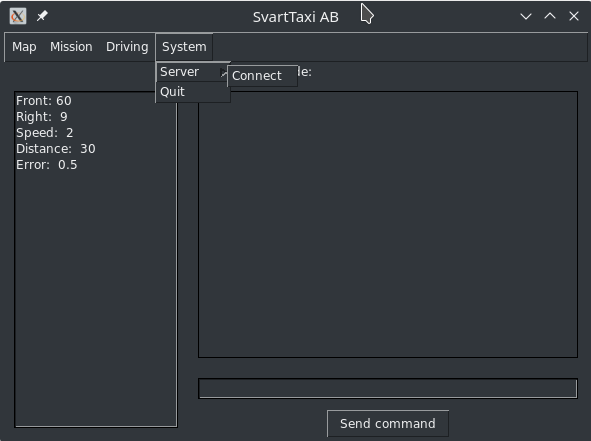
\includegraphics[width=0.6\linewidth]{\figures/system_menu.png}
    \caption{Hur man navigerar för att ansluta till servern.}
    \label{fig:sys_menu}
\end{figure}

\noindent
Efter att man tryckt på Connect kommer en ruta upp där
man kan skriva in en IP-adress.

\begin{figure}[H]
    \centering
    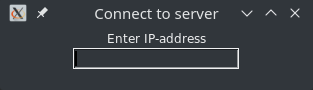
\includegraphics[width=0.6\linewidth]{\figures/enter_ip.png}
    \caption{Rutan som kommer upp när man trycker på \textit{Connect}.}
    \label{fig:connect}
\end{figure}

\noindent
IP-adressen som ska skrivas in är samma IP-adress bilen är uppkopplad till. För
att bekräfta sitt val av IP måste enter-knappen på tangentbordet tryckas ner.
Ett meddelande skrivs ut i terminalen efter att man trycker på enter, med ett
felmeddelande ifall klienten inte lyckas anslutas till bilen

\subsection{Körning}
Efter att ha anslutit till bilen kan man välja ifall man vill styra bilen
manuellt eller ifall man vill att bilen skall köra autonomn. För att välja
detta navigerar man till Driving-Manual respektive Driving-Auto.

\begin{figure}[H]
    \centering
    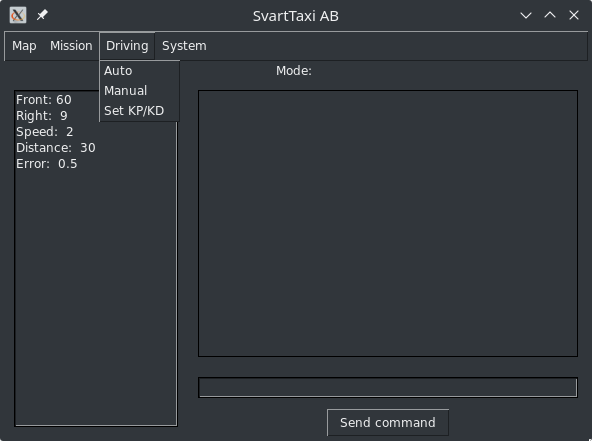
\includegraphics[width=0.6\linewidth]{\figures/driving_menu.png}
    \caption{Hur man navigerar för att byta körläge.}
    \label{fig:driving_mode}
\end{figure}

\noindent
För att ändra reglerparametrarna navigerar man till Driving-Set KP/KD. En ny
ruta kommer upp där man kan ange värden för parametrarna man vill ändra. För
att bekräfta sitt val av KP/KD måste man, precis som tidigare, trycka ner
enter-knappen på tangentbordet.

\subsection{Banan}
Banan representeras av noder och enkelriktade kanter, där varje nod
representerar en stopp-, rondell- eller parkeringslinje på banan. Varje kant
representerar en vägfil på banan. För att skapa noder högerklickar man i den
stora rutan på gränssnittet och navigerar till Create. Där finns flera olika
valalternativ. Man kan välja antingen Stopline, Parking, Inner, Outer eller
Empty. Se Figur \ref{fig:create_node}.

\begin{figure}[H]
    \centering
    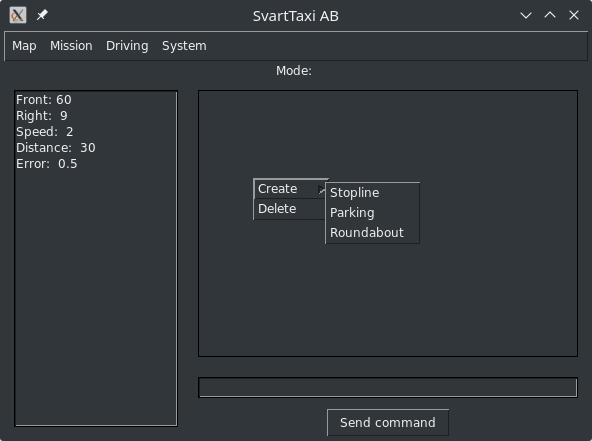
\includegraphics[width=0.6\linewidth]{\figures/create_node_menu.png}
    \caption{Hur man navigerar för att skapa olika noder.}
    \label{fig:create_node}
\end{figure}
 
\noindent
Stopline-noder är representerade av röda cirklar, Parking av gula
cirklar, Inner av mörkblå cirklar, Outer av ljusblå cirklar och Empty av vita
cirklar. Se Figur \ref{fig:node_colors}

\begin{figure}[H]
    \centering
    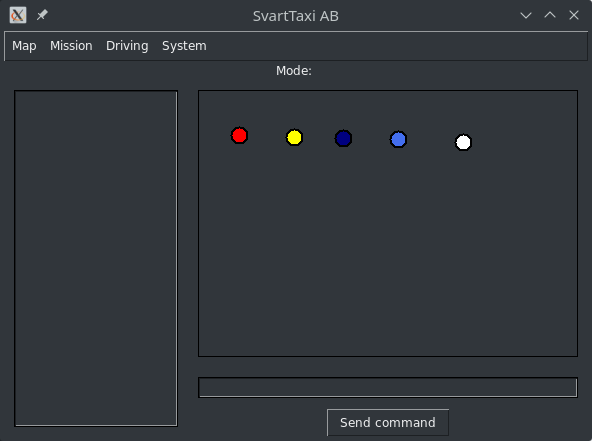
\includegraphics[width=0.6\linewidth]{\figures/node_colors.png}
    \caption{Noder med olika färger.}
    \label{fig:node_colors}
\end{figure}

\noindent
För att skapa kanter måste man först ha skapat 2 noder. Om man vänsterklickar
på en nod blir den grön, detta betyder att noden är markerad. Om man
vänsterklickar på en annan nod medan en nod är markerad kommer en ny ruta upp
där man kan mata in kostnaden på kanten. Kostnaden representerar längden på
vägfilen i banan. Alla kanter är riktande åt endast ett håll.

\begin{figure}[H]
    \centering
    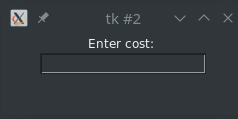
\includegraphics[width=0.6\linewidth]{\figures/enter_cost.png}
    \caption{Rutan som kommer fram när man ska skapa en kant.}
    \label{fig:create_edge}
\end{figure}

\noindent
Rondeller på banan representeras en nod för varje infart till rondellen (Outer)
och en nod för varje utfart från rondellen (Inner). för att skapa en giltig
varje utfart (Inner). En rondell med 3 infarter/utfarter representeras med 6
noder, en rondell med 4 infarter/utfarter representeras med 8 noder, och så
vidare. En rondell med 4 utfarter kan se ut som visat i Figur
\ref{fig:roundabout}, där även kanterna är dragna.

\begin{figure}[H]
    \centering
    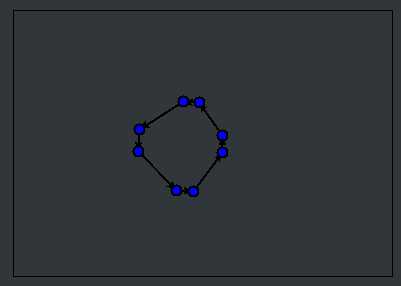
\includegraphics[width=0.6\linewidth]{\figures/roundabout.png}
    \caption{Exempel på en rondell.}
    \label{fig:roundabout}
\end{figure}

\noindent
De vita noderna används för att fylla ut kartan så att den ger en närmare
representation av verkligheten.  Ett exempel på hur en bana ser ut visas i
Figue \ref{fig:course}

\begin{figure}[H]
    \centering
    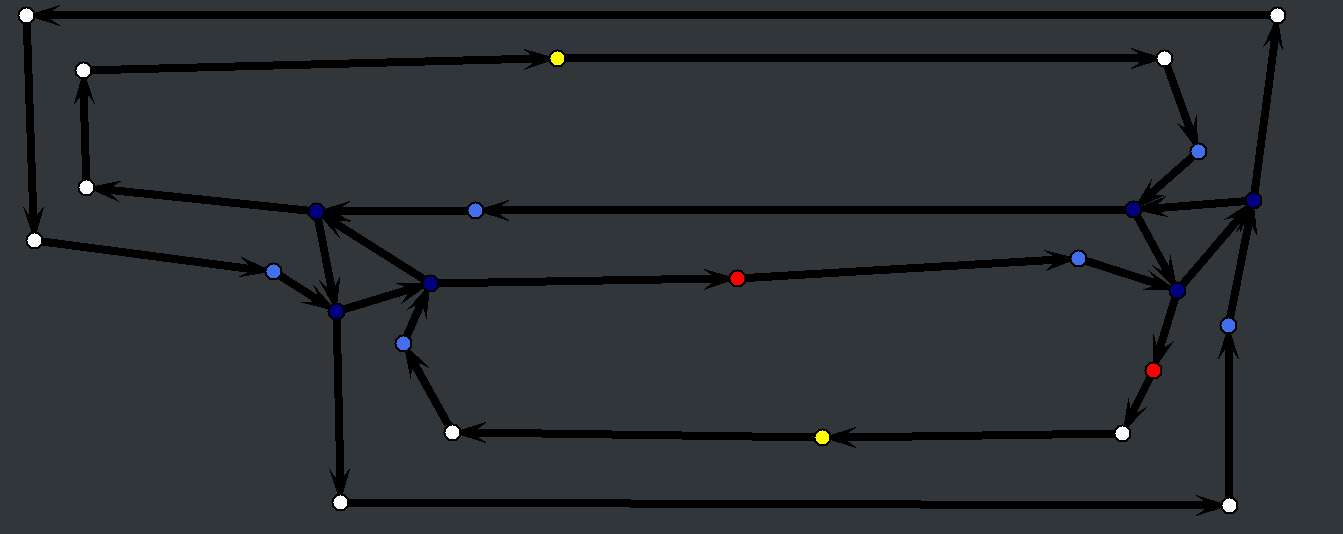
\includegraphics[width=0.6\linewidth]{\figures/course.png}
    \caption{Exempel på en fullständig karta.}
    \label{fig:course}
\end{figure}

\subsection{Uppdrag}
För att starta ett uppdrag navigerar man till Mission-Set mission och sedan
trycker man på noden man vill starta uppdraget i, följt av noden man vill
avsluta uppdraget i. Uppdraget borde endast sättas medan bilen är i manuellt
körläge. För att sedan utföra uppdraget autonomn sätter man körläget till Auto.

\begin{figure}[H]
    \centering
    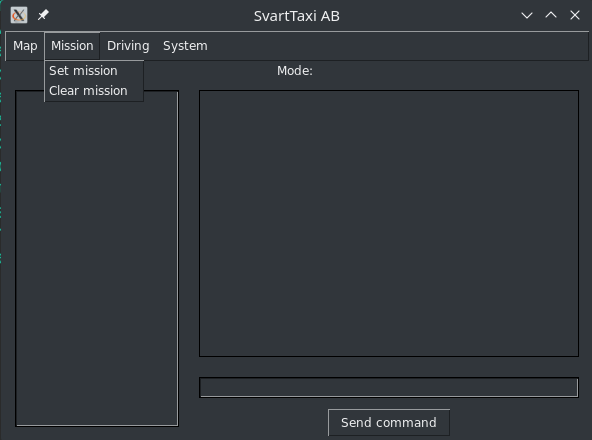
\includegraphics[width=0.6\linewidth]{\figures/set_mission.png}
    \caption{Hur man navigerar för att bestämma ett uppdrag.}
    \label{fig:set_mission}
\end{figure}

\noindent
Om man vill skapa ett längre uppdrag, så skapar man deluppdragen separat, och
sedan sätter man bilen i körläget Auto. Ett uppdrag som exempelvis A-B-C-D,
matas in som 3 separata uppdrag; A-B, B-C och C-D.

För att rensa ett satt uppdrag navigerar man till Mission-Clear mission.

\subsection{Position i banan}
För att utmärka vilken position bilen är i på banan så lyses bågen bilen är på
upp på kartan i rosa färg. Varje gång bilen passerar en linje på banan så
ändras positionen genom att nästa segment lyses upp. För ett exempel på hur det
ser ut när positionen visas, se Figur \ref{fig:pos}

\begin{figure}[H]
    \centering
    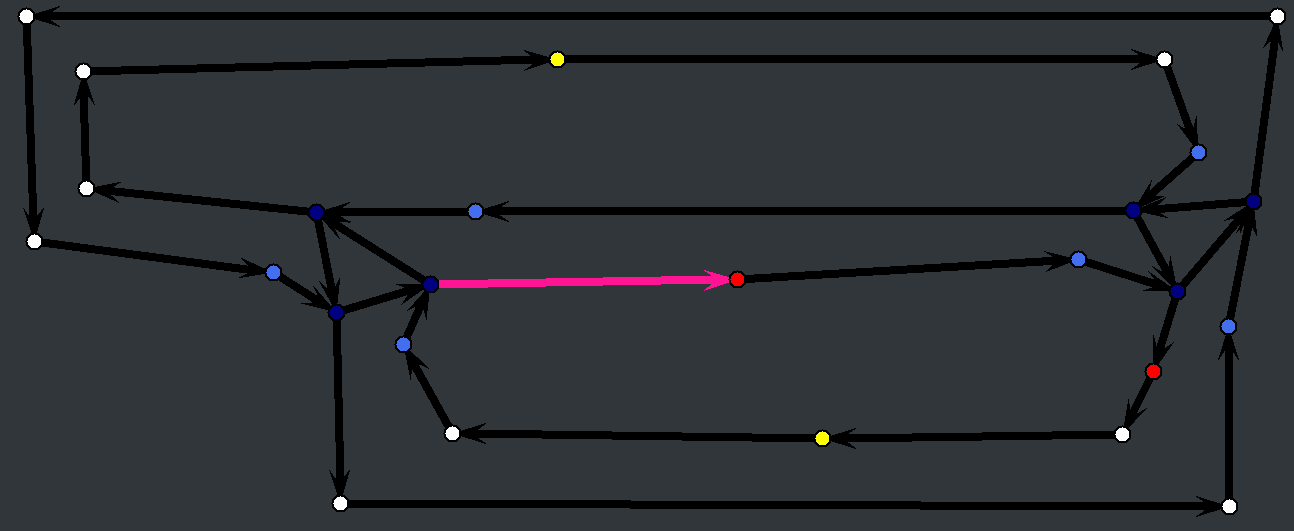
\includegraphics[width=0.6\linewidth]{\figures/pos.png}
    \caption{Hur man navigerar för att bestämma ett uppdrag.}
    \label{fig:pos}
\end{figure}
